% o \label{codigo} serve para podermos fazer referencias para algo numerado, 
% como capitulos, tabelas, figuras, etc. 
% Quando colocamos o comando \ref{codigo}. o compilador troca o \ref{codigo}
% pelo numero atribuido ao \label{}
% ex. \label{tabelaLegal}
%   A tabela \ref{tabelaLegal} mostra que...
% vai ser substituido por
%   A tabela 2 mostra que

\chapter{Roteiro de Testes}\label{cap-roteiro-testes}

Para a avaliação da eficácia do produto final deste trabalho, uma extensa 
sessão de \textit{playtesting} foi realizada, contemplando principalmente
representantes do público alvo escolhido - crianças entre 8 e 12 anos de 
idade. As experiências dos jogadores conforme observadas e relatadas foram 
então compiladas em um relatório descrevendo os aspectos positivos e negativos 
do jogo, bem como dificuldades técnicas encontradas.

\TODO{Temos que falar que fizemos tbm o roteiro, checamos com crianças da idade para ver o vocabulario, e validamos com profissionais da area}

% ---
\section{Playtesting}\label{sec-playtesting}
% ---

A seção de \textit{playtesting} foi realizada durante o Tech Kids Day 
realizado no museu Catavento Cultural no dia 12 de novembro como parte 
da São Paulo Tech Week 2016. 

Uma versão reduzida e simplificada do jogo foi elaborada, contendo uma 
parcela suficientemente representativa do conteúdo do jogo, enquanto 
mantendo o tempo de jogo dentro de um período de 15 minutos ou menos, 
compatível com as condições de teste.

\begin{figure}[h]
	\centering
	\caption{crianças testando o jogo durante a no Tech Kids Day}
	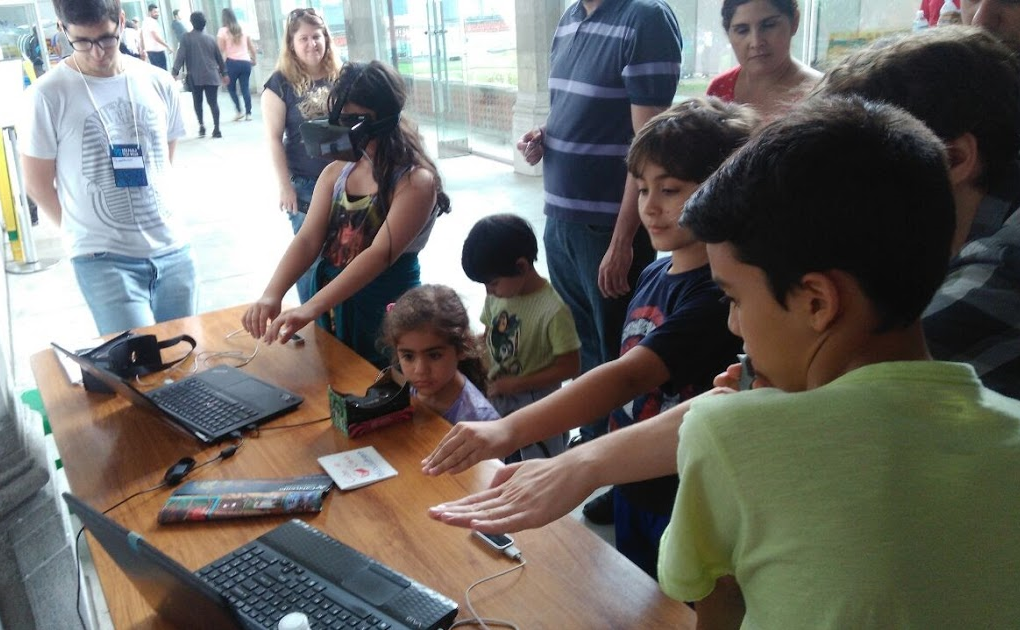
\includegraphics[width=0.5\textwidth]{tech_kids_booth}
	\legend{\fonteAP}
	\label{fig:tech-kids-day}
\end{figure}

Essa versão consiste em um conjunto de 4 fases, dispondo do seguinte conteúdo:

\begin{alineas}
	\item \textbf{Fase 1:} introdução ao funcionamento básico do jogo. Apresentação das mecânicas de seleção em área e manipulação da elevação do terreno;
	\item \textbf{Fase 2:} introdução de mecânicas de criação e manipulação de corpos d'água.
	\item \textbf{Fase 3:} introdução da mecânica de vento e da criação de blocos de areia.
	\item \textbf{Fase 4:} combinação de todos os elementos apresentados em um cenário mais complexo
\end{alineas}

Duas cópias do jogo foram iniciadas lado a lado, uma ligada tanto 
ao \textit{Leap Motion} para controle gestual quanto ao \textit{Cardboard} 
para o efeito de realidade virtual, como pode ser visto 
na \autoref{fig:tech-kids-day}, enquanto outra ligada apenas ao 
\textit{Leap Motion}, com o \textit{output} direto pela tela do computador, 
mostrado na \autoref{fig:tech-kids-day-pc}.

\begin{figure}[h]
	\centering
	\caption{jogo sendo executado apenas com o \textit{Leap Motion}}
	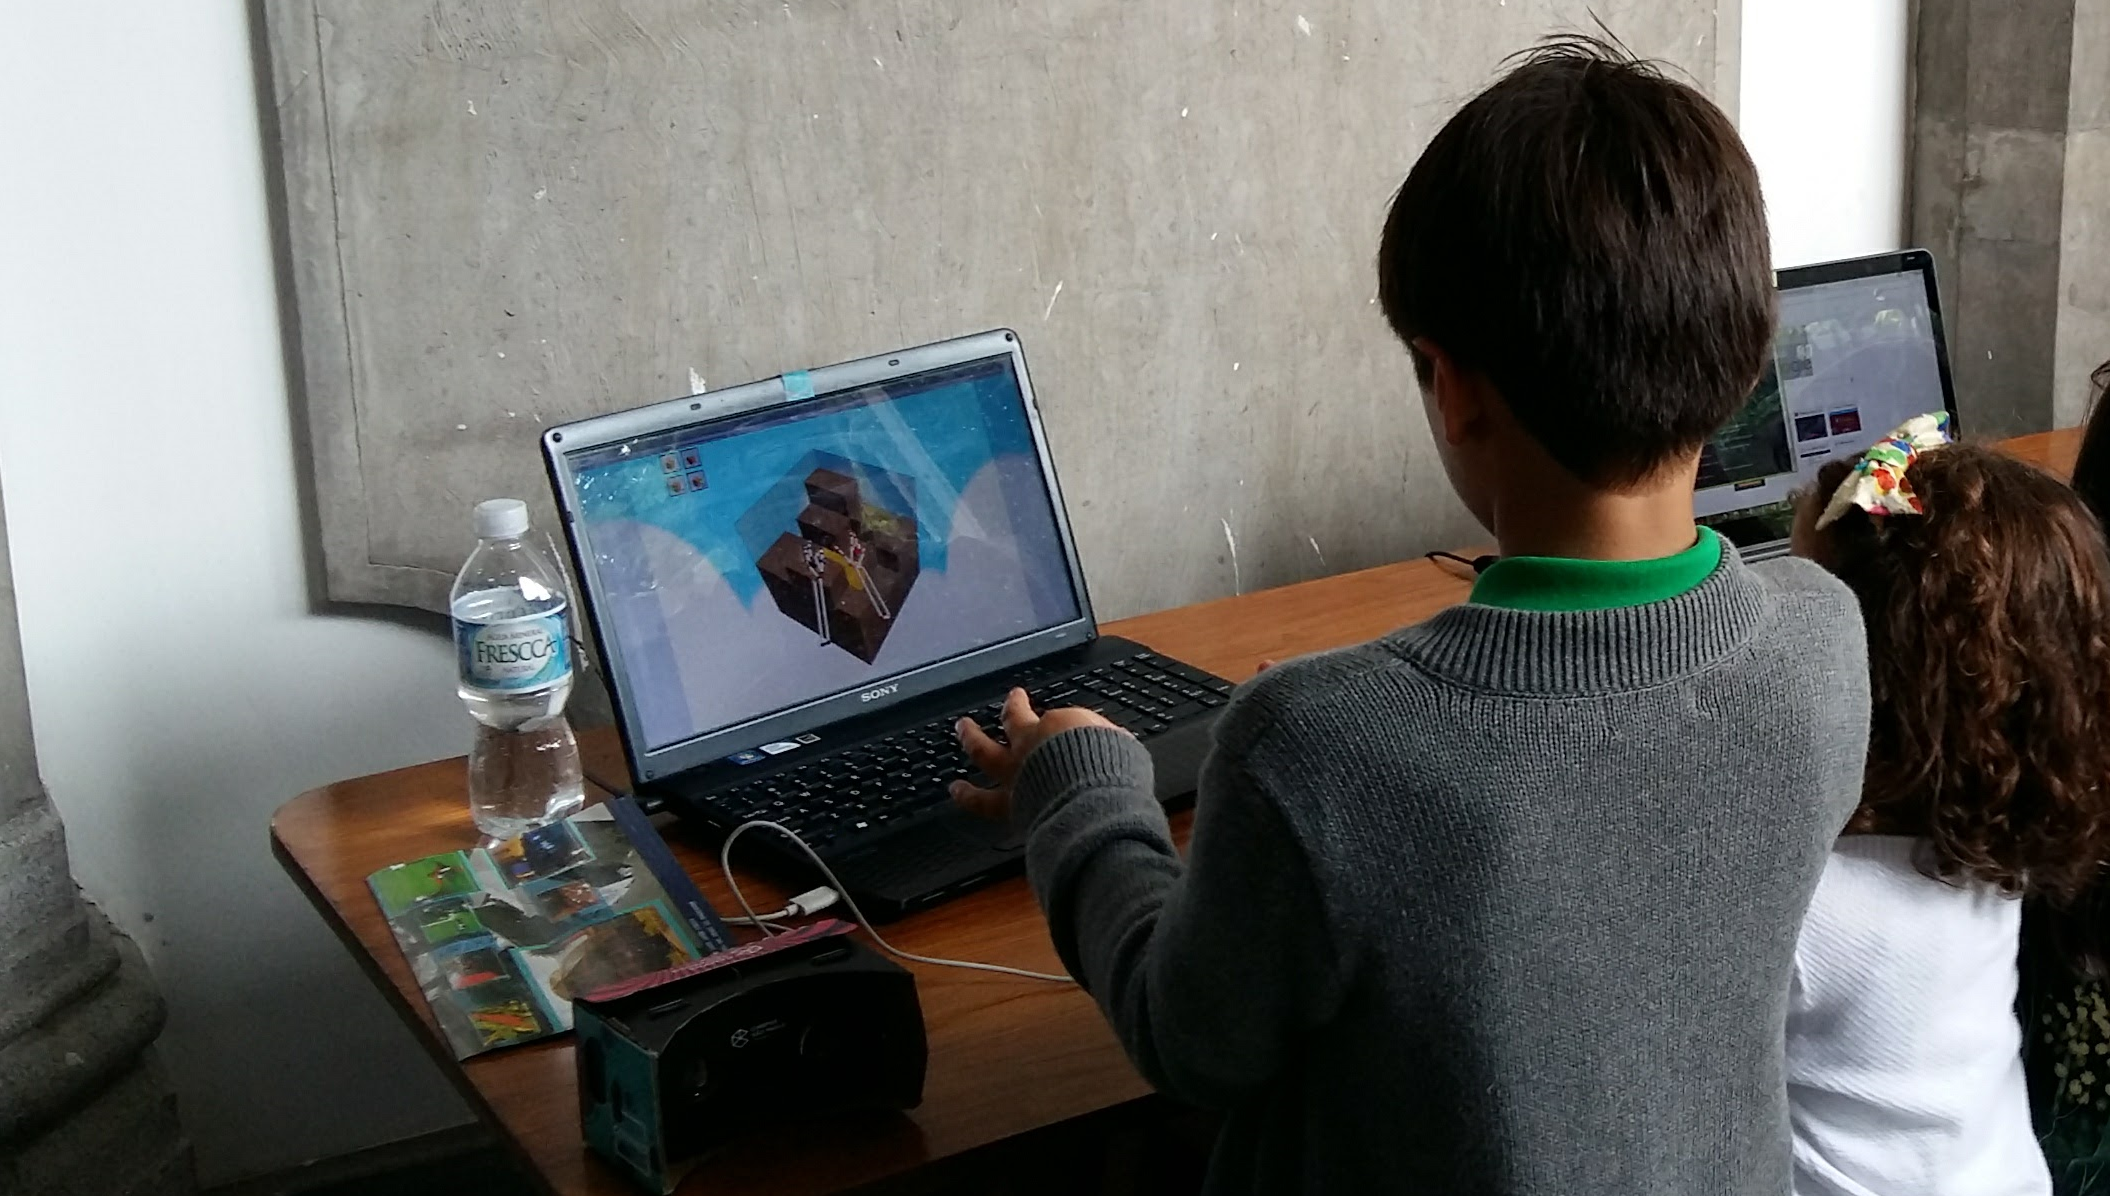
\includegraphics[width=0.5\textwidth]{tech_kids_booth2}
	\legend{\fonteAP}
	\label{fig:tech-kids-day-pc}
\end{figure}

Durante a execução do \textit{playtesting} foi notada a reação dos 
jogadores e seu \textit{feedback} foi coletado após cada sessão do jogo, 
conforme descrito na \autoref{sec-roteiro-observacoes}

\section{Observações}\label{sec-roteiro-observacoes}

Os resultados dos testes, obtidos através da observação e do 
\textit{feedback} dos jogadores, trouxeram à tona problemas inesperados, 
bem como pontos positivos na implementação escolhida.

Em termos gerais, o jogo foi bem recebido pelas crianças, que se 
mostraram e entretidas durante todos os 15 minutos de sessão. Ficou claro 
também que a versão executando em realidade virtual foi mais popular, 
despertando bastante interesse nos jogadores.

Contudo, algumas interações mecânicas se revelaram mais difíceis de se 
executar do que era esperado, exigindo uma familiaridade com os sensores 
que fugia ao escopo do tempo de teste. Sobretudo as mecânicas de gerar e 
remover água se comportaram de maneira menos responsiva do que necessário 
para que o jogo pudesse ser jogado com naturalidade.

Em termos técnicos, os sensores utilizados no projeto apresentaram 
dificuldades em detectar os gestos e movimentos executados por crianças 
mais novas, devido tanto à incapacidade do \textit{Leap Motion} em 
reconhecer mãos pequenas quanto à impossibilidade das crianças em 
manter confortavelmente as mão à altura necessária para a captura 
correta de seus movimentos. 

Adicionalmente, o ambiente não colaborou com a seção de testes. A mesa 
aonde estavam dispostos os jogos se encontrava muito iluminada por 
fontes de luz, por estar do lado de uma janela. Visto que o controlador 
funciona com a captura de imagens infravermelhas, o excesso de luz 
diminuiu a qualidade de captura do controlador, interferindo no jogo.

Apesar dos desafios encontrados, a experiência geral se mostrou 
positiva, e o \textit{feedback} obtido será muito valioso para desenvolver 
iterações do projeto.

\TODO{Checar se deixamos "Será" ou "foi"}